\documentclass[a4paper]{article}

\usepackage[T2A]{fontenc}
\usepackage[utf8]{inputenc}
\usepackage[russian]{babel}
\usepackage{graphicx}
\usepackage{float}
\usepackage{mathtools}
\usepackage{wrapfig}
\usepackage{amsfonts, amssymb, amsmath, latexsym}
\usepackage{nicefrac}
\usepackage{hhline}
\usepackage{multirow}
\usepackage[colorlinks=true,linkcolor=blue,citecolor=blue]{hyperref}       % hyperlinks
\usepackage{nicefrac}       % compact symbols for 1/2, etc.
\usepackage{nameref}
\usepackage{booktabs}       % professional-quality tables
\usepackage{algorithm}
\usepackage{algpseudocode}
\usepackage{xcolor, colortbl}
\usepackage{etoolbox}
\usepackage{tikz}

% \graphicspath{ {./} }

\usepackage[verbose=true,letterpaper]{geometry}

\newgeometry{
    textheight=25cm,
    textwidth=18cm,
    top=2.5cm,
    headheight=12pt,
    headsep=10pt,
    footskip=1cm,
    marginparwidth=15pt
}

%\usepackage{showframe} 

\usepackage{epigraph}
\usepackage{amsmath,amsfonts,amssymb,amsthm,mathtools, mathrsfs}
\usepackage{amsthm}

\title{Работа 4.7.2 \\ Эффект Поккельса}
\author{Шарапов Денис, Б05-005}
\date{}

\usepackage{fancyhdr}
\pagestyle{fancy}
\fancyhf{}
\rhead{Работа 4.7.2}
\lhead{}
\cfoot{\thepage}
\usepackage{subcaption}
\usepackage[font={small}]{caption}

\begin{document}

    \maketitle
    \tableofcontents
    \newpage
    
\section{Аннотация}

\noindent\textbf{Цель работы:} исследовать интерференцию рассеянного света, прошедшего кристалл; наблюдать изменение характера поляризации света при наложении на кристалл электрического поля.\smallskip
 
\noindent \textbf{В работе используются:} гелий-неоновый лазер, поляризатор, кристалл ниобата лития, матовая пластина, экран, источник высоковольтного переменного и постоянного напряжения, фотодиод, осцилограф, линейка.

\section{Теоретические сведения}

Эффект Поккельса --- изменение показателя преломления света в кристалле под действием электрического поля. \medskip

\noindent Рассмотрим кристалл ниобата лития $\text{LiNbO}_3$ с цетрольноосевой симметрией вдоль оси $Z$. Для световой волны с $\mathbf{E}$ перпендикулярно $Z$ показатель преломления будет $n_o$, а для волны с $\mathbf{E}$ вдоль $Z$ --- $n_e$. В случае, когда луч света идёт под углом $\theta$ к оси, есть два значения показателя преломления $n_1$ и $n_2$: $n_1 = n_o$ для волны с $\mathbf{E}$ перпендикулярным плоскости $(\mathbf{k},\mathbf{Z})$ (обыкновенная волна) и $n_2$ для волны с $\mathbf{E}$ в этой плоскости (необыкновенная волна). В последнем случае

\begin{equation}
\dfrac{1}{n_2^2}=\dfrac{\cos^2 \theta}{n_0^2}+\dfrac{\sin^2 \theta}{n_e^2}.
\end{equation}

\noindent Если перед кристаллом, помещённым между поляроидами, расположить линзу или матовую пластинку, то на экране за поляроидом мы увидим тёмные концентрические окружности --- результат интерфернции обыкновенной и необыкновенной волн. При повороте выходного поляроида на $90^\circ$ картина меняется с позитива на негатив (на месте светлых пятен тёмные и наоборот). В случаи, когда разрешённое направление анализатора перпендикулярно поляризации лазерного излучения, радиус тёмного кольца с номером $m$ равен

\begin{equation}
r_m^2 = \dfrac{\lambda}{l} \dfrac{(n_oL)^2}{n_0 - n_e}m,
\end{equation}

\noindent где $L$ --- расстояние от центра кристалла до экрана, $l$ --- длина кристалла. \medskip


\noindent Теперь поместим кристалл в постоянное электрическое поле $E_{\text{эл}}$, направленное вдоль оси $X$, перпендикулярной $Z$. Показатель преломления для луча, распространяющего вдоль $Z$, всегда $n_o$. В плоскости $(X,Y)$ возникают два главных направления под углами $45^\circ$ к $X$ и $Y$ с показателями преломления $n_0 - \Delta n$ и $n_o + \Delta n$ (быстрая и медленная ось), причём $\Delta n = A E_{\text{эл}}$. Для поляризованного вертикально света и анализатора, пропускающего горизонтальную поляризацию, на выходе интенсивность на выходе будет иметь вид

\begin{equation}
I_{\text{вых}} = I_0 \sin^2 \left(\dfrac{\pi}{2} \dfrac{U}{U_{\lambda/2}} \right),
\end{equation}

\noindent где $U_{\lambda/2} = \frac{\lambda}{4A}\frac{d}{l}$ -- \textit{полуволновое напряжение}, $d$ -- поперечный размер кристалла.  При напряжении $U = E_{\text{эл}}d$ равном полуволновому сдвиг фаз между двумя волнами равен $\pi$, а интенсивность света на выходе максимальна. 

\section{Результаты измерений и обработка данных}
\subsection{Исследование интерференции рассеянного света}

\begin{figure}[ht!]
    \centering
    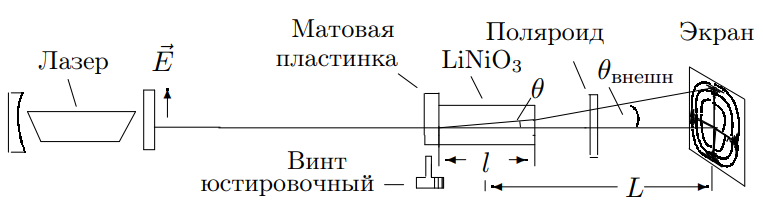
\includegraphics[width = 0.52\textwidth]{image/pic1.png}
    \caption{Схема для наблюдения интерференционной картины}
\end{figure}

\noindent В схеме, изображенной на рис. 1 получим интерфереционную картину. Измерим радиусы $r(m)$ тёмных колец при расстоянии $L = 60$ см и результаты запишем в таблицу 1. На рис. 2 изобразим график зависимости $r^2 =~f(m)$.

\begin{figure}[ht!]
    \centering
    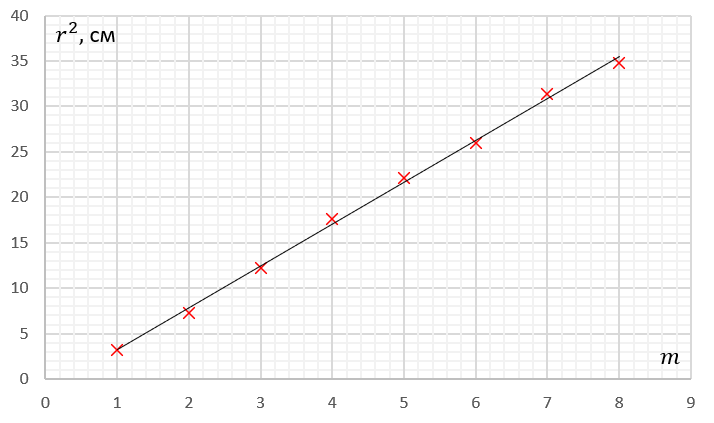
\includegraphics[width = 0.52\textwidth]{image/graph.png}
    \caption{График зависимости квадрата радиуса кольца от порядка минимума}
\end{figure}

\noindent Из МНК получим угловой коэффициент $$k = 4,36 \pm 0,04 \;\; \text{см}^2.$$ Откуда при значениях из таблицы 1 получим $$n_0 - n_e = 0,11 \pm 0,01.$$

\subsection{Изменение характера поляризации света при наличии внешнего поля}

\begin{figure}[ht!]
    \centering
    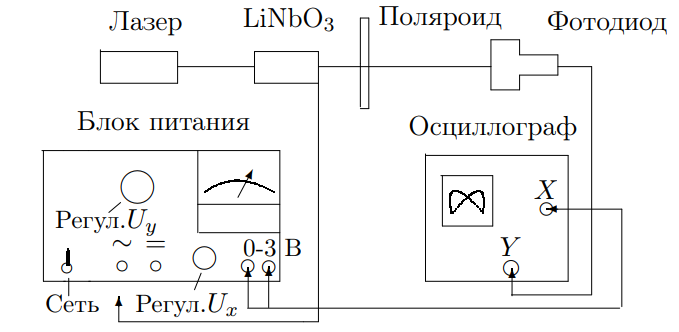
\includegraphics[width = 0.55\textwidth]{image/pic2.png}
    \caption{Схема для изучения двойного лучепреломления в электрическом поле}
\end{figure}

\noindent Для скрещенных поляризаций при напряжениях $U = (2k - 1)U_{\lambda/2}$ наблюдается максимум интенсивности, при $U = 2kU_{\lambda/2}$ - минимум, здесь $k$ - натуральное число. Для параллельных поляризаций ситуация противоположная. 
	
\noindent Напряжения, соответствующие последовательным экстремумам интенсивности для разных поляризаций, содержатся в таблице 3. В 100 делениях шкалы блока питания 1,5 кВ. Погрешность измерения напряжения примем равной 1 делению, или 15 В. \medskip

\noindent По таблице 3 найдем среднее значение полуволнового напряжения; погрешность его определения складывается из приборной погрешности и случайной, сопоставимых по величине, поэтому оценим ее как $2\cdot 10$ В: $$U_{\lambda / 2} \approx 30 \text{ дел} = 450 \text{ В}.$$

\section{Вывод}

Рассмотрен эффект Поккельса: несколькими способами определено полуволновое напряжение, оно совпадает в пределах погрешности и равно $U_{\lambda/2} \approx 460$ В. Получены фигуры Лиссажу, отражающие зависимость интенсивности выходного сигнала от подаваемой амплитуды напряжения $I(U)$ при скрещенных и параллельных поляризациях. Картинки для поляризаций отличаются по фазе на $\pi/2$.

\section{Приложение}

\begin{table}[!ht]
    \centering
    \caption{Параметры установки}
    \begin{tabular}{|c|c|c|}
    \hline
    $n_0$  & $\lambda$, мкм & $l$, мм \\ \hline
    $2,29$ & $0,630$        & $26$    \\ \hline
    \end{tabular}
\end{table}

\begin{table}[!ht]
    \centering
    \caption{Радиусы темных колец при расстоянии $L = 60$ см}
    \begin{tabular}{|c|c|c|c|c|c|c|c|c|}
    \hline
    $m$     & 1     & 2     & 3     & 4     & 5     & 6     & 7     & 8     \\ \hline
    $r$, см & $1,8$ & $2,7$ & $3,5$ & $4,2$ & $4,7$ & $5,1$ & $5,6$ & $5,9$ \\ \hline
    \end{tabular}
\end{table}


\begin{table}[ht!]
    \centering
    \caption{Измерение последовательных напряжений, соответствующих минимумам/максимумам интенсивности для скрещенных и параллельных поляризаций}
    \begin{tabular}{|c|c|c|}
        \hline
        &Скрещенные поляризации&Параллельные поляризации\\
        \hline
        $U_{\lambda/2}$, дел&30&28\\
        \hline
        $U_{\lambda/2}$, В&450&420\\
        \hline
        \hline
        $2U_{\lambda/2} = U_\lambda$, дел&60&60\\
        \hline
        $2U_{\lambda/2} = U_\lambda$, В&900&900\\
        \hline
        \hline
        $3U_{\lambda/2} = U_{3\lambda/2}$, дел&92&92\\
        \hline
        $3U_{\lambda/2} = U_{3\lambda/2}$, В&1380&1380\\
        \hline
    \end{tabular}
\end{table}

\begin{figure}[ht!]
    \begin{minipage}[h]{0.3\linewidth}
        \center{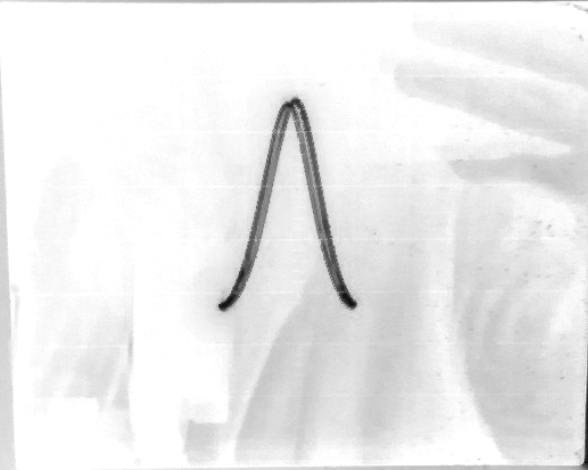
\includegraphics[width=0.9\linewidth]{image/photo1.png} \\ a)}
    \end{minipage}
    \hfill
    \begin{minipage}[h]{0.3\linewidth}
        \center{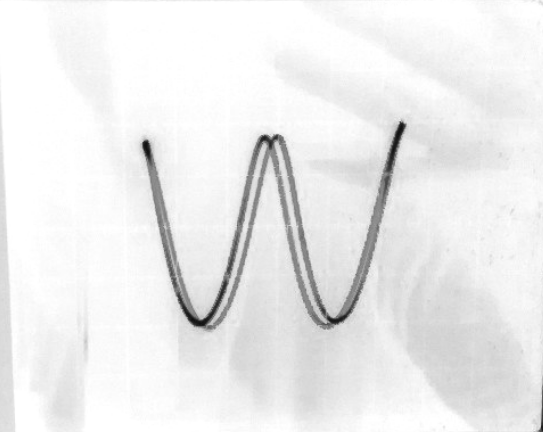
\includegraphics[width=0.9\linewidth]{image/photo2.png} \\ b)}
    \end{minipage}
    \hfill
    \begin{minipage}[h]{0.3\linewidth}
        \center{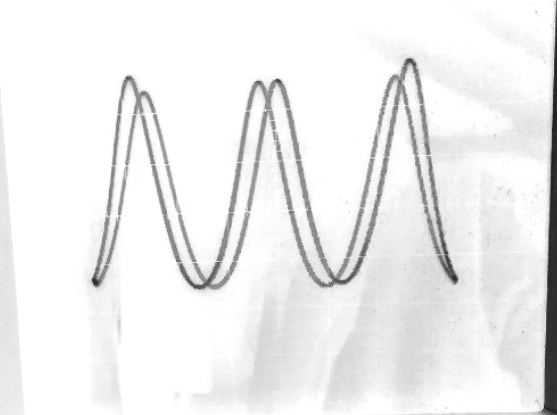
\includegraphics[width=0.9\linewidth]{image/photo3.png} \\ c)}
    \end{minipage}
    \caption{Фигуры Лиссажу для параллельных поляризаций при различных амплитудах напряжения $U$: (a) $U = U_{\lambda/2}$, (b) $U = U_{\lambda}$, (c) $U = U_{3\lambda/2}$ }
    \label{lis}
\end{figure}

\end{document}
